\documentclass[11pt]{article}
\usepackage{geometry}
\geometry{
a4paper,
lmargin=2cm,
rmargin=2cm,
tmargin=2cm,
bmargin=2cm
}
\usepackage{float}
\usepackage{indentfirst}
\usepackage{caption}
\usepackage{graphicx}
\usepackage{listings}
\usepackage{color}
\usepackage[T1]{fontenc}
\lstloadlanguages{C,C++,csh,Java}

\definecolor{red}{rgb}{0.6,0,0}
\definecolor{blue}{rgb}{0,0,0.6}
\definecolor{green}{rgb}{0,0.8,0}
\definecolor{cyan}{rgb}{0.0,0.6,0.6}

\renewcommand{\contentsname}{Sadržaj}

\lstset{
	language=csh,
	basicstyle=\footnotesize\ttfamily,
	numbers=left,
	numberstyle=\tiny,
	numbersep=5pt,
	frame=box,
	tabsize=2,
	extendedchars=true,
	breaklines=true,
	stringstyle=\color{blue}\ttfamily,
	showspaces=false,
	showtabs=false,
	xleftmargin=17pt,
	framexleftmargin=17pt,
	framexrightmargin=5pt,
	framexbottommargin=4pt,
	commentstyle=\color{green},
	morecomment=[l]{//}, %use comment-line-style!
	morecomment=[s]{/*}{*/}, %for multiline comments
	showstringspaces=false,
	morekeywords={ abstract, event, new, struct,
	as, explicit, null, switch,
	base, extern, object, this,
	bool, false, operator, throw,
	break, finally, out, true,
	byte, fixed, override, try,
	case, float, params, typeof,
	catch, for, private, uint,
	char, foreach, protected, ulong,
	checked, goto, public, unchecked,
	class, if, readonly, unsafe,
	const, implicit, ref, ushort,
	continue, in, return, using,
	decimal, int, sbyte, virtual,
	default, interface, sealed, volatile,
	delegate, internal, short, void,
	do, is, sizeof, while,
	double, lock, stackalloc,
	else, long, static,
	enum, namespace, string},
	keywordstyle=\color{cyan},
	identifierstyle=\color{black},
	backgroundcolor=\color{white},
}

\title{Domaći 3 - Servis HMI i PLC}
\author{Ognjen Čavić E2 161/2024}
\date{Novembar 2024}
\begin{document}
\maketitle
\section{Opis problema}
Panel (ili HMI) se pretplaćuje na PLC pomoću metode \textbf{InitHMI}, gde se
navodi koju promenljivu želi da prati.
PLC je dužan da šalje informaciju o novoj vrednosti promenljive svakih 15
sekundi, gde panel te vrednosti iscrtava "grafički".
Ukoliko se od PLC-a traži da šalje vrednost promenljive koja ne postoji, on
šalje nulu, specifikacija problema to ne zahteva, ali rešenje implementira
mogućnost da ako se ta promenljiva pojavi, PLC će početi da je šalje.
\section{Logika rešenja}
Kada HMI pošalje navede koju promeljivu želi da prati tako što navede adresu
ili naziv, u \textbf{InitHMI} se prvo određuje da li je poslata adresa ili 
naziv.
Adrese se odlikuju time što počinju sa "prefiksom" \textbf{ADDR} koji je praćen
brojem.
Nakon toga se unutar servisa panelu dodeljuje identifikacioni broj kako bi se
oni razlikovali, te se kreira instanca klase \textbf{Panel} koja se upisuje
u rečnik \textbf{panels} i callback funkcija tog procesa se upisuje u drugi
rečnik \textbf{panelCallbacks}.
Bitno je reći da se rečnici mogu zameniti nizovima i postiči istu funkcionalnost,
ali ovakav pristup je manje sklon greškama.
\par Publisher tj. PLC treba da na svakih 15 sekundi pošalje nove vrednosti
promenljivih svim pretplaćenim panelima.
Na početku \textbf{Publish} metode se kreira lista \textbf{idsToNotify} sa
identifikacionim brojevima (ID) svih pretplaćenih panela.
Potom se generiše nasumičan broj za svaku od promenljivih koji se šalje svakom
panelu, čiji identifikacioni broj se uklanja iz liste nakon slanja.
Slanje poruke podrazumeva pozivanje odgovarajuće callback funkcije, prosleđivanje
argumenata koji predstavljaju poslate informacije.
Ukoliko je neki panel pretplaćen na nepostojeću promenljivu, njegov ID ostaje
u listi nakon završetka petlje, u drugoj petlji se svim panelima koji nisu 
dobili poruku šalje nula.
\par Callback funkcija se bavi "grafičkim" prikazom primljenih informacija tako
što ih čuva u nizu \textbf{data} i za svaki član tog niza crta odgovarajući broj
vertikalnih crtica.
\textbf{GRAPH\_OFFSET} je konstanta kojom se graf pomera nekoliko mesta u desno
kako bi se napravilo mesta za skalu.
Ovde ta skala poprilični jednostvna, broj 0 skroz dole i broj 100 skroz
gore dok se između njih ispisuje poslednja pristigla vrednost na odgovarajučoj
visini.
Glavna stvar u crtanju koja pravi probleme je činjenica da y-osa raste u
suprotnom smeru u odnosu na Dekartov koordinanti sistem, stoga stvari moraju
biti prilagođene drugačije. 
\section{Rezulati}
Kada se pokrenu servis, panel i plc (PLC i Panel mogu da se pokrenu u
proizvoljnom redosledu i neće doći do izuzetka) u konzoli aplikacije za panel
se unosi promenljiva koja treba da se prati.
Kada se \textbf{initHMI} izvrši i počne slanje poruka panelu, on počinje da ih
iscrtava kako pristižu.
\par Na slici 1 se nalazi primer iscrtanog grafika, gde su vrednosti prikazane
odgovarajućim crtama, nova vrednost je prikazana na odgovarajućoj visini.
Na slici 2 se nalazi više grafika, tj pokrenuto je više panela, gde je svaki
pretplaćen na različitu promenljivu.
\begin{center}
	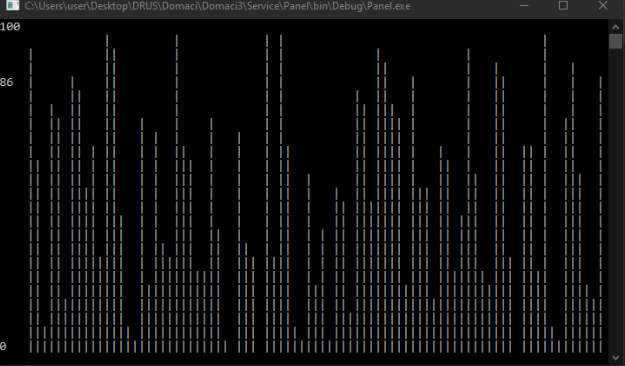
\includegraphics[scale=1]{figs/jedan_grafik.PNG}
	\captionof*{figure}{Slika 1: Primer grafika}
\end{center}
\begin{center}
	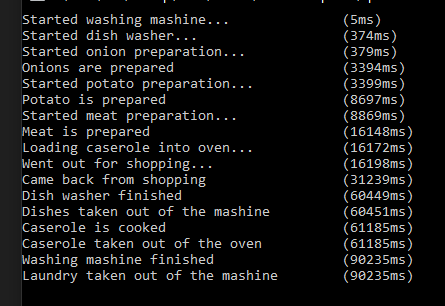
\includegraphics[scale=0.44]{figs/Rezultat.PNG}
	\captionof*{figure}{Slika 2: Primer više grafika}
\end{center}
\end{document}
